\subsection[Einleitung]{Einleitung \myAuthor{Jonas Leitner}} \label{sec:solver_intro}

Als Solver standen wir vor dem Auftrag, ein in Form von Bildern digitalisiertes Puzzle so zu lösen, dass es anschließend vom Roboter richtig zusammengesetzt werden kann. 
Dabei sahen wir uns mit einer Reihe von Problemen konfrontiert. Jedes Bild repräsentiert genau ein Puzzleteil. Zum einen muss das Bild so verarbeitet werden, dass die jeweiligen Kanten (Edges) der Puzzleteile extrahiert werden können. In einem weiteren Schritt ist es notwendig, ein Vergleichsmaß zu erhalten, mit dem zwei Kanten auf Ähnlichkeit verglichen werden können. Diese zwei Schritte haben wir auch als Preprocessing definiert. Mit diesen Informationen kann dann ein Algorithmus entwickelt werden, der die richtige Anordnung der Puzzleteile in einer Matrix löst. Dabei ist zu beachten, dass die Puzzleteile in Schritten von 90 Grad gedreht werden können. So weiß man nach dem Lösungsalgorithmus die genaue Anordnung der Puzzleteile und welche Kante zu welcher gehört.

Das Puzzle ist damit aber noch nicht zusammengesetzt. Hierfür ist ein Postprocessing-Schritt notwendig, in dem die genaue Position berechnet wird, damit sich die Teile korrekt überlappen.
Eine Übersicht des Prozesses ist auch in \autoref{fig:solver_overview} visualisiert.

\begin{figure}[H] 
\centering 
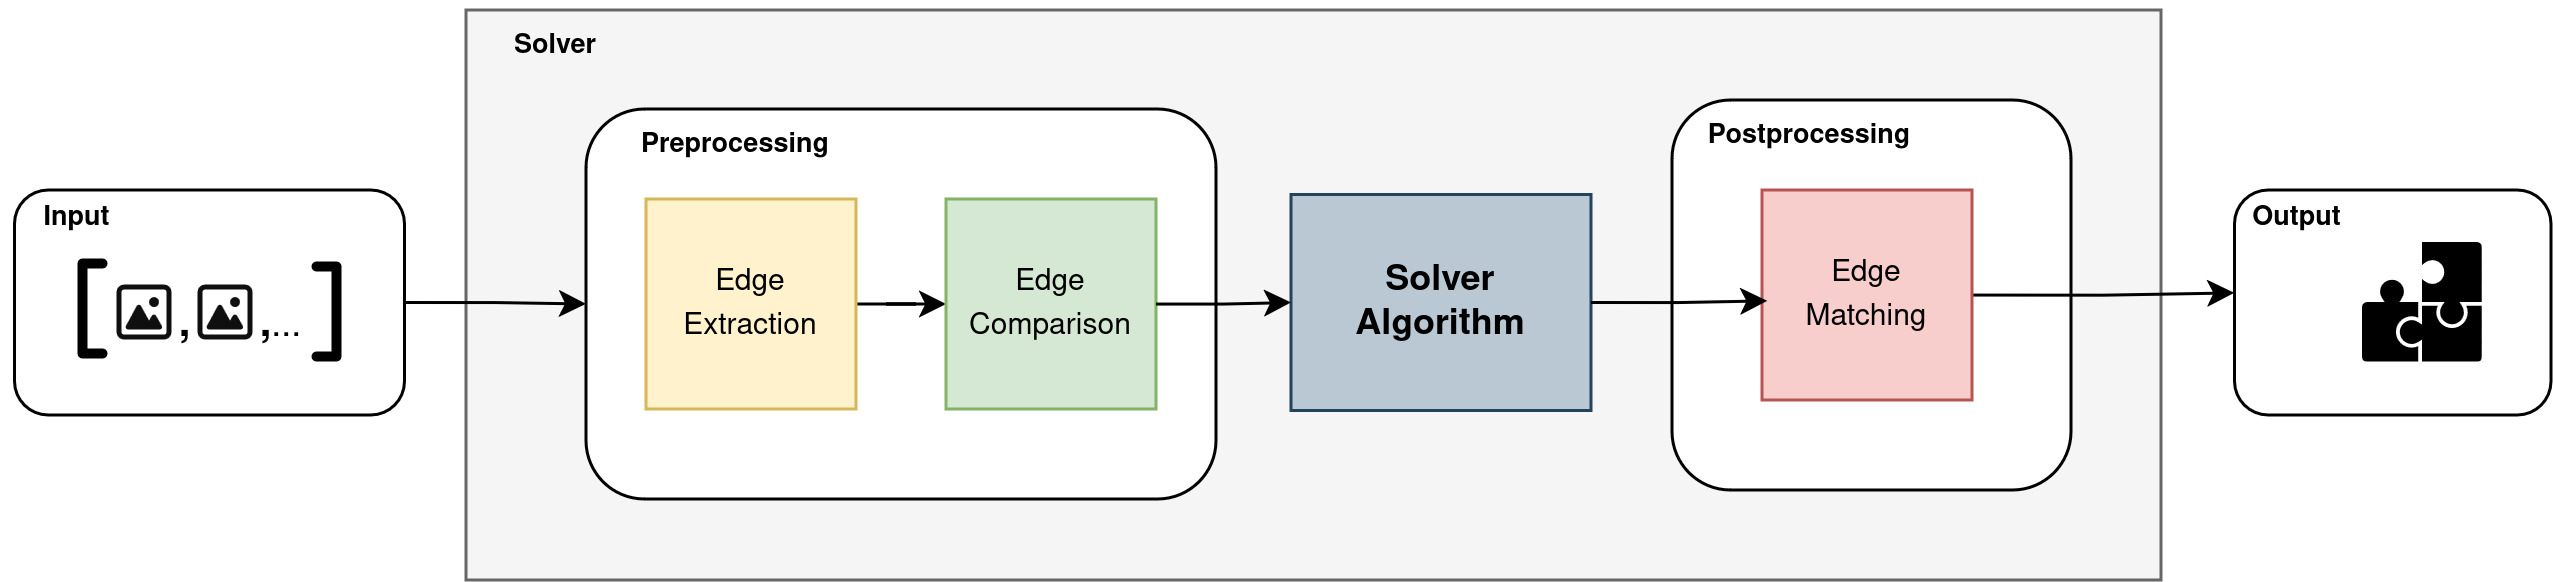
\includegraphics[width=\textwidth]{images/solver_overview.jpg} 
\caption{Übersicht des Solver Prozesses} 
\label{fig:solver_overview} 
\end{figure}

\paragraph{Klassenstruktur}

Es wurde eine Klassenstruktur konzipiert um die Handhabung zu erleichtern und Abstraktion der einzelnen Problematiken zu erreichen. Ein Überblick erleichtert im Folgenden die Verständlichkeit der einzelnen Abschnitte.

Den Kern bilden die Klassen $Puzzle$, $PuzzlePiece$ und $Edge$. Ein $PuzzlePiece$ setzt sich stets aus exakt vier Edges zusammen. Jede $Edge$ ist durch eine eindeutige ID, einen Pfad, welcher die Kante beschreibt, sowie zwei Ecken, an denen die Kante anschließt, charakterisiert. Zusätzlich wird jeder $Edge$ ein Type zugewiesen. Eine Kante kann entweder als „FLAT”, „MALE” oder „FEMALE” definiert werden. 


\begin{figure}[H] 
\centering 
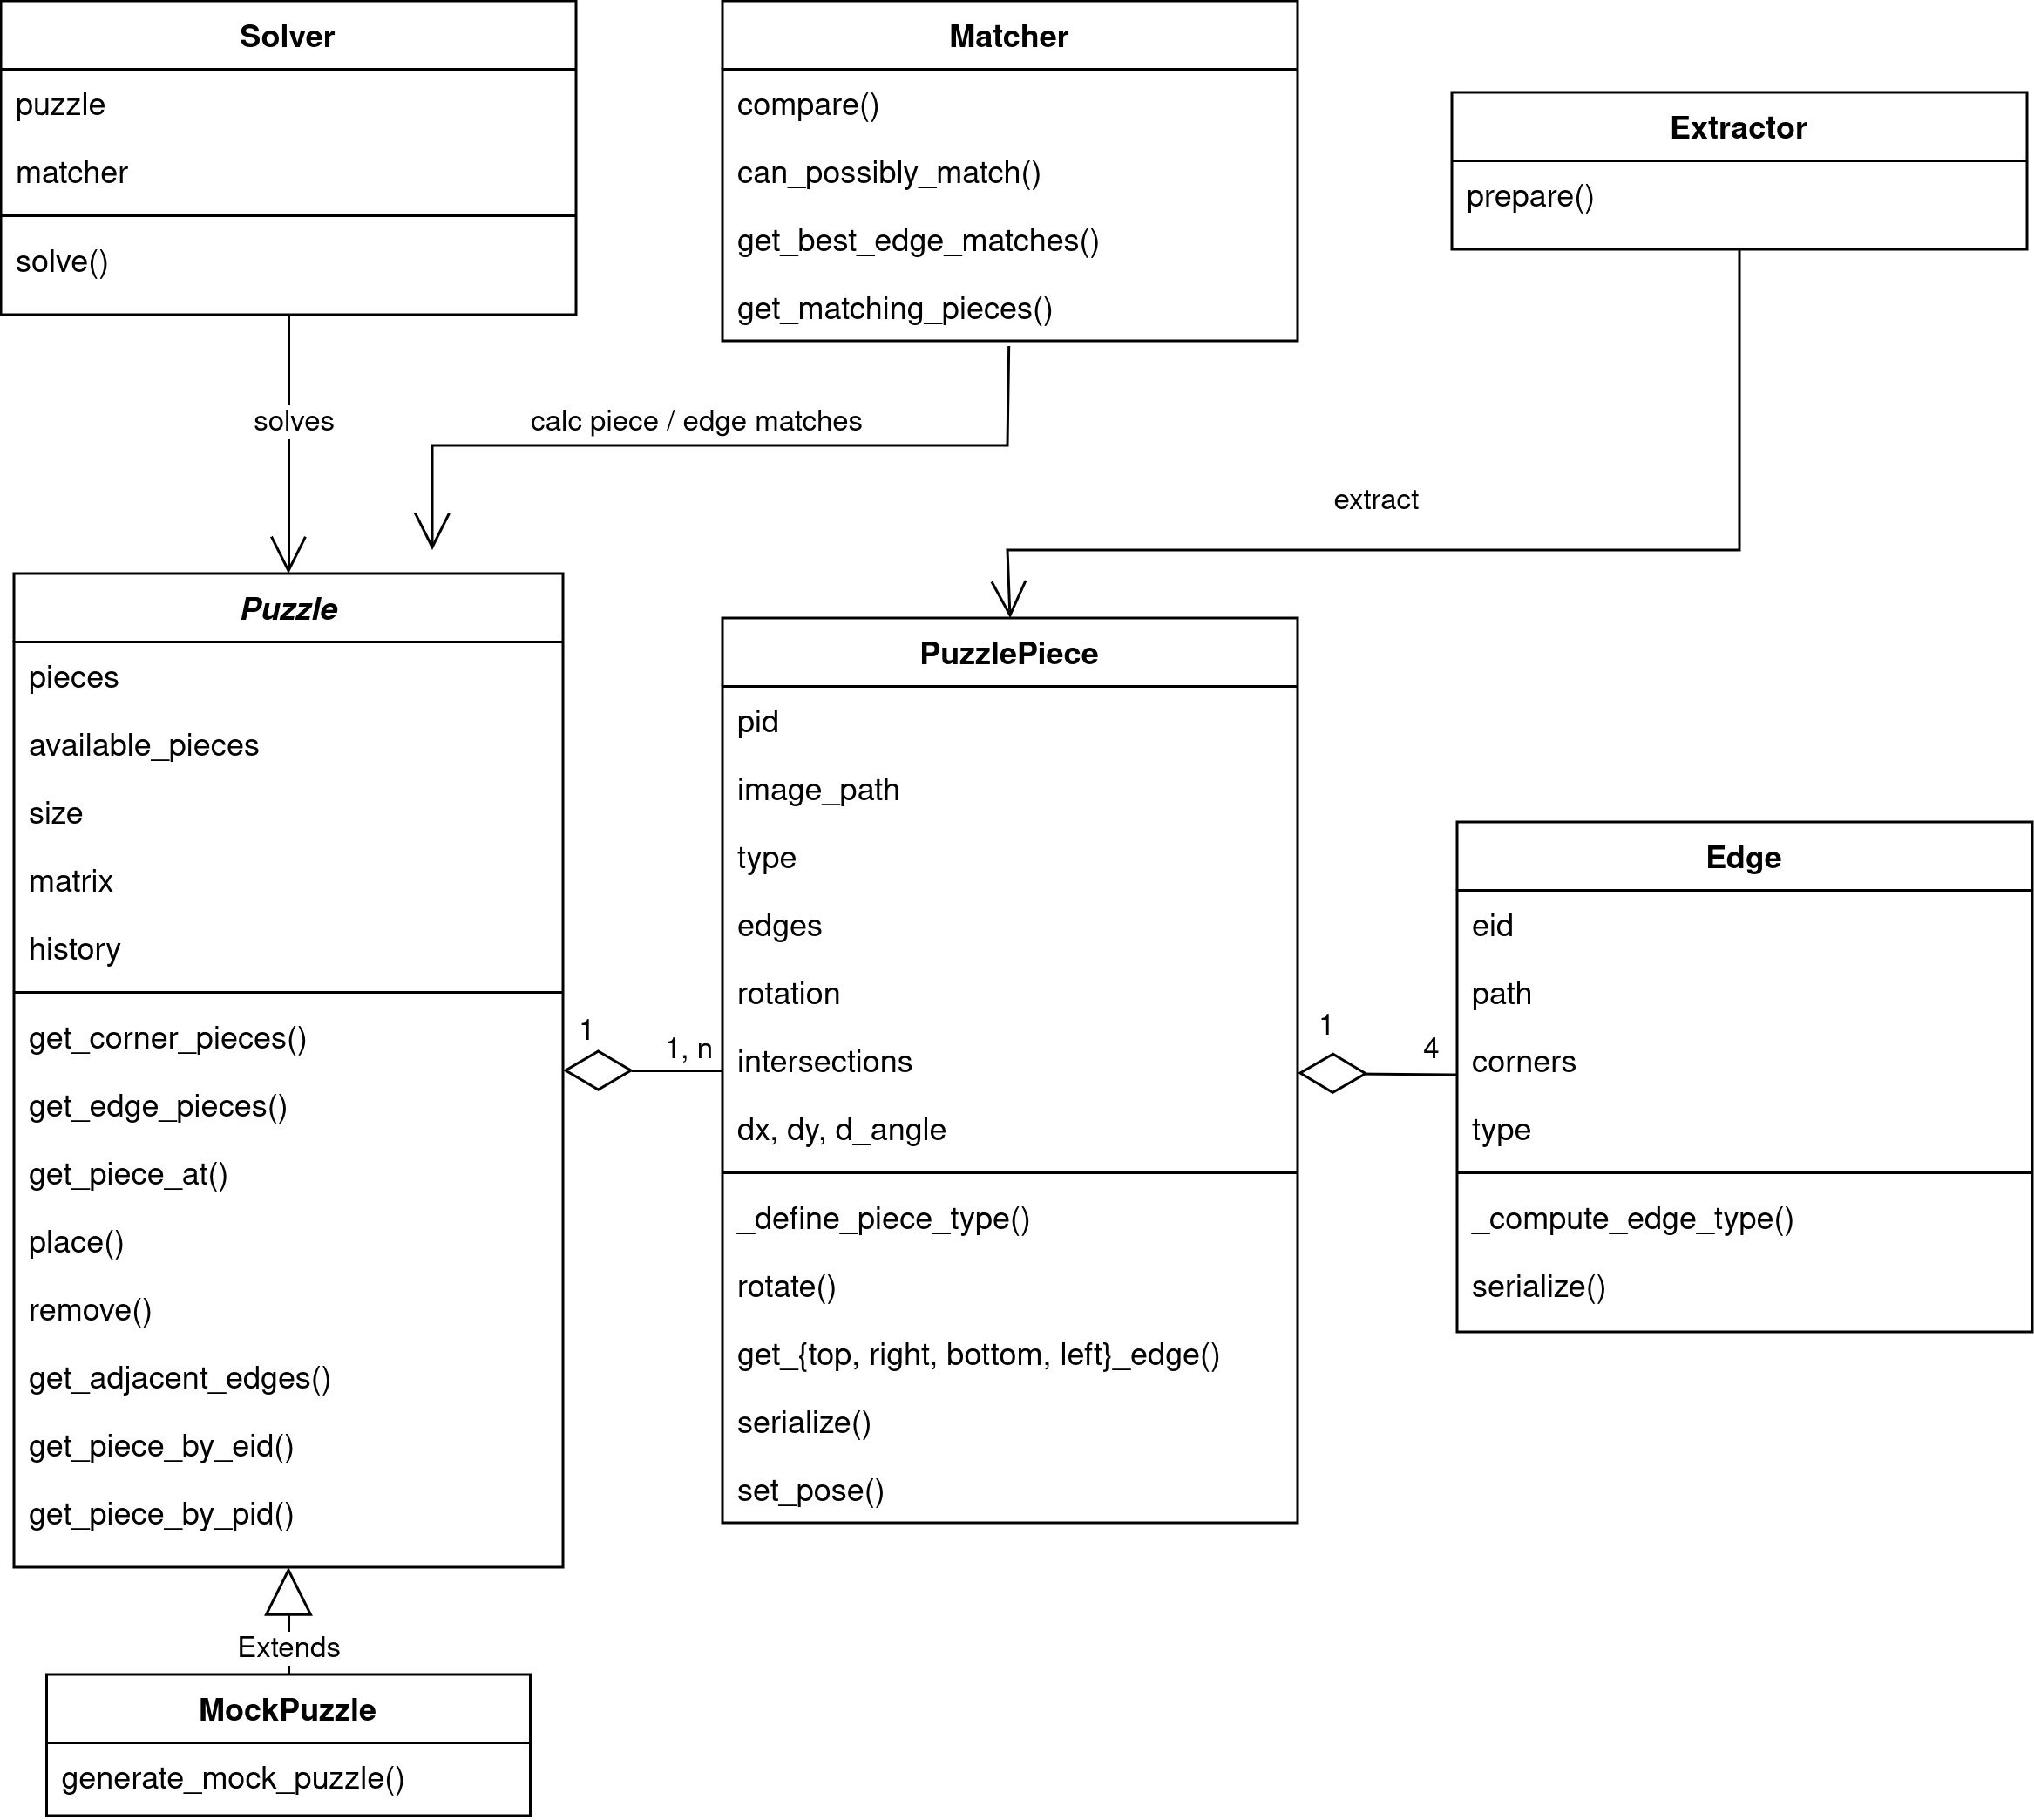
\includegraphics[width=\textwidth]{images/class_diagram.jpg} 
\caption{Vereinfachtes Klassendiagram} 
\label{fig:solver_class_diagram} 
\end{figure}

Das $PuzzlePiece$ verfügt ebenfalls über eine ID sowie einen Type. Der Type wird über die Types der dazugehörigen Edges bestimmt. Sind zwei der Kanten „FLAT”, dann handelt es sich um eine „CORNER”. Ist eine der Kanten „FLAT”, handelt es sich um ein „EDGE” Piece. Ansonsten ist der Type „DEFAULT”. Jedes $PuzzlePiece$ verfügt über einen Pfad zum dazugehörigen Bild des Puzzleteils. 
Das Attribut „edges” beinhaltet eine Liste mit vier Kanten, welche im Uhrzeigersinn angeordnet sind. Dabei stellt die erste Kante die obere dar. 
Ein Puzzleteil kann um 90, 180 und 270 Grad rotiert werden. Dabei rotiert die Position der Edges natürlich auch mit. Zusätzlich verfügt das $PuzzlePiece$ über Intersections, welche die Schnittpunkte der Hough Transformation halten. Diese werden im Postprocessing benötigt, um die exakte x-, y-Position und genaue Gradverdrehung des Puzzleteils zu berechnen. 
% Erwähnenswert ist, dass die EIDs der Edges über die PID der dazugehörigen Pieces berechnet wird. Als Beispiel: Die Edges des Piece mit PID 0 haben EIDs von 0-3. Bei Puzzleteil 1 hat die EIDs 4-7 usw. Hierduch kann immer aus der Edge ID die Piece ID zurückgerechnet werden.

Der sogenannte $Extractor$ hat die Aufgabe, eine Liste von Eingabebildern in eine Liste von definierten Puzzleteilen zu verwandeln. Der genaue Ablauf wird in \autoref{sec:extractor} beschrieben. Da der Extraktionsschritt eine gewisse Zeit in Anspruch nehmen kann, verfügen $PuzzlePiece$ und $Edge$ über eine $serialize()$-Funktion, mithilfe derer die Liste an Puzzleteilen in Form eines JSON gespeichert werden kann. Somit ist es nicht erforderlich, den Extrahierungsschritt bei jedem Durchlauf auszuführen.

Die Liste der Puzzleteile kann anschließend als $Puzzle$ erweitert werden. Das $Puzzle$ speichert eine Liste aller Puzzleteile im $pieces$-Attribut. Mithilfe dieser Liste kann auch die Größe des Puzzles berechnet werden. Das Puzzle hält eine Matrix, in der die einzelnen Puzzleteile platziert werden. Platzierte Puzzleteile werden aus der $available\_pieces$-Liste entfernt. 
Das Puzzle hat zudem einige Hilfsfunktionen. Unter anderem gibt es Funktionen die es ermöglichen alle Corner-Pieces oder Edge-Pieces zu erhalten. Ein $Piece$ kann mit $place()$ an einer bestimmten Stelle innerhalb der Matrix platziert oder mit $remove()$ auch wieder entfernt werden. Des Weiteren besteht die Möglichkeit, mit $get\_adjacent\_edges()$ alle anliegenden Edges für eine spezifische Position innerhalb der Matrix zu erhalten.

Der $Matcher$ ermöglicht die Erstellung einer Match-Matrix, welche sämtliche Kanten eines Puzzles beinhaltet. Beim Erstellen werden alle MALE und FEMALE Kanten miteinander verglichen. 
Der Matcher ist eine Basisklasse. Es existieren unterschiedliche Implementierungen des Matchers, wobei sich die $Matcher$ in der $compare()$-Funktion hinsichtlich der Berechnung des Ähnlichkeitswertes von zwei Edges unterscheiden.
In \autoref{sec:matcher} werden die einzelnen Matcher ausführlich betrachtet.
Zudem beinhaltet der Base-Matcher Hilfunktionen um beispielsweise für eine bestimmte $Edge$ eine sortierte Liste der am Besten dazu passenden $Edges$ zu erhalten.

Die Aufgabe des $Solver$ ist es dann, ein bestimmtes Puzzle mit einem ausgewählten Matcher zu lösen. Auch hier gibt es verschiedene Implementierungen des Solvers, die in \autoref{sec:solver} näher beschrieben sind.

Das $MockPuzzle$ bietet die Möglichkeit, ein Puzzle zu mocken, um die implementierten Solver besser testen zu können. Dies wird in \autoref{sec:mockpuzzle} näher erläutert.
